\section{Data Processing}

The first portion of this paper uses a considerable amount of data and is primarily restricted by both computational power and availability of a database of slums. There are five primary categories that are listed below.
\begin{itemize}
    \item \textbf{Version 4 DMSP-OLS Nighttime Lights Time Series}\textsuperscript{\cite{lightdata}}
    
    This paper uses nighttime light images from 2000 to 2013 and to reduce computational expenditure whilst also improving model relevance since most of the training data set of identified slums is from African countries in 2013. Each pixel has a resolution of one square kilometer.
    
    \begin{figure}[ht]
        \centering
        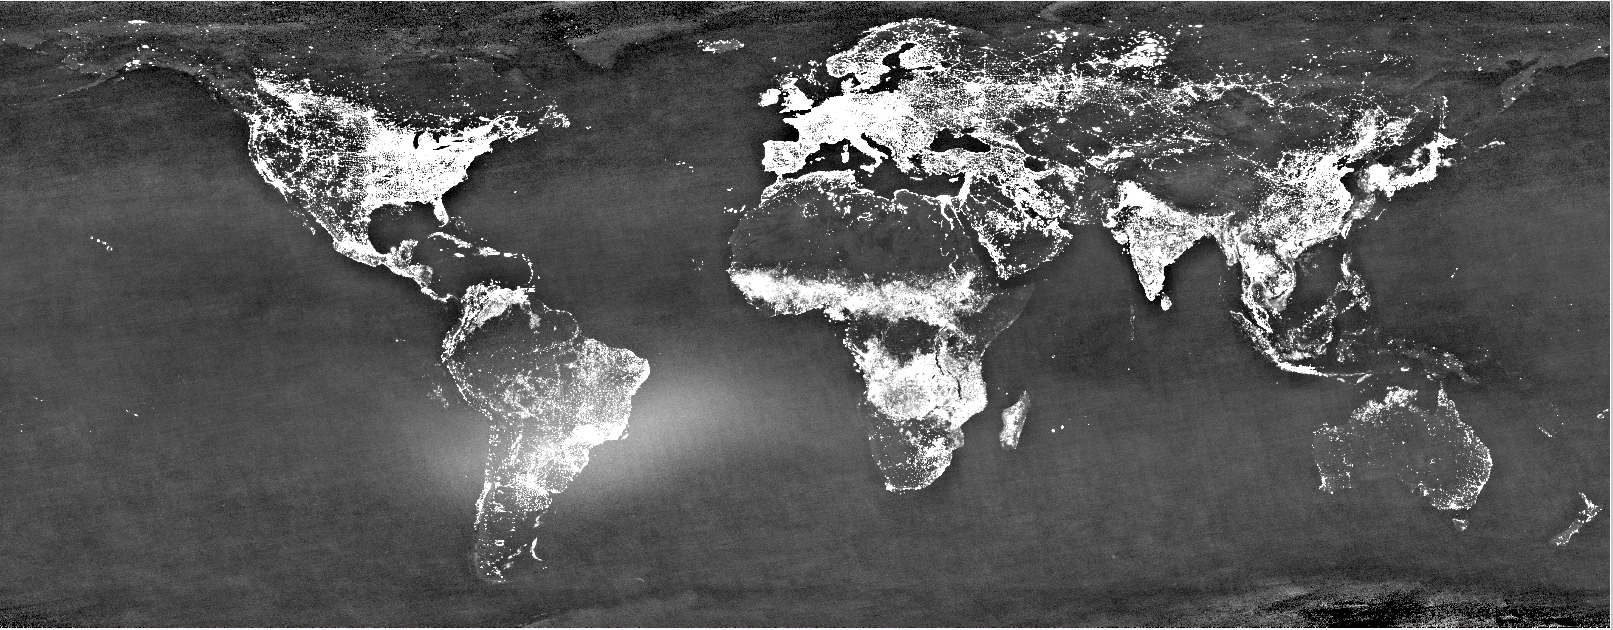
\includegraphics[scale = 0.3]{Graphics/F162008 avg lights pic.png}
        \caption{Averaged light values in 2008}
        \label{fig:F162008}
    \end{figure}
    
    This data set is the most novel out of all the other data sets in terms of usage in economics and it also requires special treatment on the processing end as well. These files are stored in a TIF format which are dense images which contain additional information at each pixel. In this case, each raw file download from NOAA contains an image of the world as below and must be processed first using spatial data processing software.    
    
    \item \textbf{World Pop Hub: Population Density Data}\textsuperscript{\cite{popdata}}
    
    The second data set that this paper is contingent on is population density. WorldPop.org is a very encompassing database that includes a granular count of population density with a resolution of 1 kilometer.
        
    \item \textbf{Slum Dwellers International}\textsuperscript{\cite{slumdata}}
    
    This data set acts as the training data set that includes already identified slums, their coordinates, and additional characteristics of the slum such as access to sanitation or public transportation. This data does not exist in a consolidated format and must be scraped from SDI.org. This information was collected by consulting locals to survey areas from 2013 to 2018 in cities that are widely considered by locals to be slums.

    \item \textbf{World Bank: World Development Indicators}\textsuperscript{\cite{wdislums}}

    When abstracting the mapping model to multiple countries, we would use a series of world bank indicators as controls - an extensive list of potential variables is included in Table 17 in the appendix - to distinguish countries from each other. Currently, I use the WDI indicators to calibrate the household choice model using data about slum population as a proportion of total urban population in countries.

    \item \textbf{Numbeo: Rent Characteristics of Countries}\textsuperscript{\cite{Numbeo}}

    This data set is also used to calibrate the household choice model. It consists of the aggregate results of surveys of various cities across countries which report on characteristics such as income and rent - among many others.
    
\end{itemize}

 Several decisions had to be made about the scope of the lights and population density data to consider since although data was plenty in these two areas, the slums data set was very limited. Making assumptions that the slums data set had profiled all the slums in a given country would drastically skew models as there might be many areas that are slums in real life and whose light and population density characteristics indicate to be so but are not captured in the slums data set. As such, lights and population density observations were taken from grid areas around cities we know were surveyed for slums. In the future, given a more precise slums data set, this paper can be much better tuned. 

Once all the data sets are individually processed, we still must merge them all by coordinate points. This introduces another set of assumptions. The first issue is the matching of coordinate points between the nighttime lights and population density data sets. There are several methods of conducting this matching process that vary in time complexity and accuracy. After conducting a time complexity and accuracy tradeoff analysis, this paper conducts the matching process by creating larger pixel grids, calculating the average population density of each larger grid space, and then assigning that new aggregate population density value to each of the smaller pixels within that larger grid unit. In addition, to classify coordinate points as slums or not, we have to do a similar process of first making a simplifying assumption that slums are spatially circular in nature and translate the square meter area into distance difference in geo-coordinates. This area to geo-coordinate translation also includes another simplifying assumption in that we disregard the curvature of the earth; this assumption, however, is minute and often taken as a given when working with physical areas as small as the ones in the slums data set. Once the radius of each slum is identified, calculating whether a geo-coordinate pair in the lights data set is regarded to be a slum is a simple issue of calculating if distance to the center of any of the documented slums is less than that given slum's radius.






